
\section{Modélisation mathématique du problème}
Notre modelisation mathematique commence par le choix des outils mathematiques utilises ( \textbf{les graphes} ),
passe par le formalisme et les analogies et se terminent par le choix des algorithmes permettant de resourdre le probleme.\\

Cependant,justifons d'abord le choix de la \textbf{theorie des graphes}
\begin{enumerate}
    \item Tout d'abord,nous devons souligner que la theorie des graphes est un outil simple,facile a comprendre et qui illustre mieux comment representer une carte,des routes et autres.
    \item De plus,le probleme que nous devons resourdre s'assimile directemnet aux poblemes de parcours en  theorie des graphes
    \item par ailleurs,La théorie des graphes offre des outils puissants pour modéliser les connexions entre les différents points du réseau routier et les déplacements des véhicules d'un point à un autre.
\end{enumerate}




% ------------------------------------------------------
\subsection{Un peu de théorie des graphes}
A fin de faciliter la comprehension de notre modele,nous allons bievrement definir expliquer les concepts de base de la theorie des graphes utiles pour notre modelisation. 

\begin{figure}[h]
    \centering
    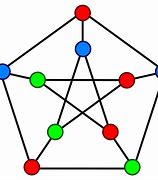
\includegraphics[width=0.5\linewidth]{Images/Theory.jpeg}
    \caption{La theorie des graphes}
    \label{fig:un peu de theorie des graphes}
    \cite{graph_image}
\end{figure}


\subsubsection{Qu'est ce que de théorie des graphes ?}

La théorie des graphes est une branche des mathématiques qui étudie les relations entre les objets. Les objets sont représentés par des points, appelés sommets, et les relations entre eux sont représentées par des lignes, appelées arêtes. Voici quelques concepts de base :

\subsubsection{Terminologie}

\begin{itemize}
    \item \textbf{Graphe :} Ensemble de sommets et d'arêtes.
    \item \textbf{Sommets (ou nœuds) :} Les points d'un graphe.
    \item \textbf{Arêtes :} Les lignes reliant les sommets.
    \item \textbf{Graphe orienté :} Un graphe dans lequel les arêtes ont une direction.
    \item \textbf{Graphe non orienté :} Un graphe dans lequel les arêtes n'ont pas de direction.
    \item \textbf{Graphe mixte :} Un graphe dans lequel certaines arêtes peuvent être orientées et d'autres non, et où les sommets peuvent être attribués à différents types ou classes.
    \item \textbf{Graphe pondéré :} Un graphe dans lequel chaque arête est associée à un poids ou une valeur. Ces poids peuvent représenter des distances, des coûts, des temps, etc., et sont utilisés pour optimiser les algorithmes de recherche de chemins tels que Dijkstra et A* qui seront presentes ci bas.
\end{itemize}


\begin{figure}[h]
    \centering
    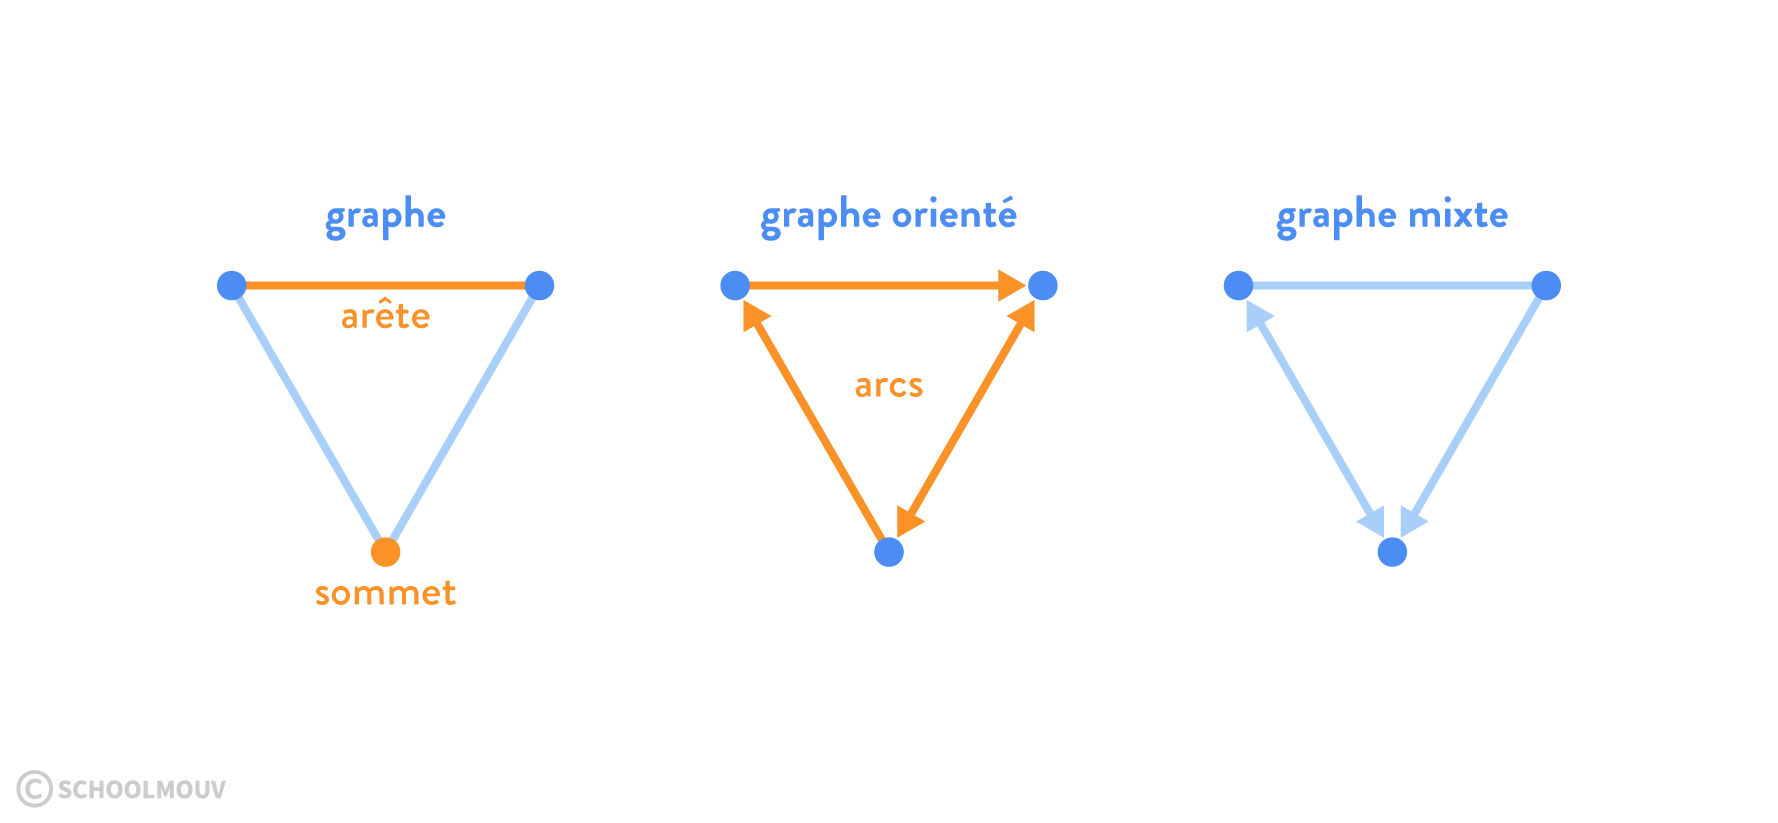
\includegraphics[width=0.9\linewidth]{Images/sommets.png}
    \caption{Terminologie theorie des graphes}
    \cite{graph_image2}
\end{figure}

\newpage
\subsubsection{Types de graphes}

Il existe plusieurs types de graphes, dont les plus courants sont :

\\
     \textbf{Graphe simple :} Un graphe sans boucles ni arêtes multiples entre les mêmes sommets.
\begin{figure}[h]
    \centering
    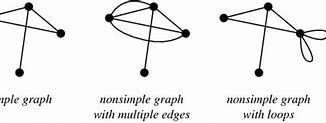
\includegraphics[width=0.4\linewidth]{Images/simple_graph.jpeg}
    \caption{graphe simple}
    \cite{graph_image3}
    \end{figure}
     
  \\   \textbf{Graphe complet :} Un graphe dans lequel chaque paire de sommets est reliée par une arête.

    \begin{figure}[h]
    \centering
    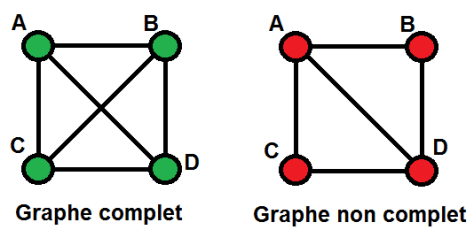
\includegraphics[width=0.4\linewidth]{Images/graph_simple_complet.png}
    \caption{graphe complet}
    
    \cite{graph_image4}
\end{figure}
    
  \\  \textbf{Graphe biparti :} Un graphe dont les sommets peuvent être divisés en deux ensembles disjoints, et où chaque arête relie un sommet d'un ensemble à un sommet de l'autre ensemble.

\begin{figure}[h]
    \centering
    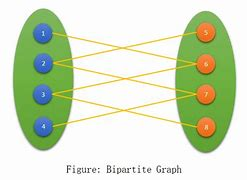
\includegraphics[width=0.4\linewidth]{Images/bipartite_graph.jpeg}
    \caption{graphe bipartite}
    % \cite{graph_image5}
\end{figure}





La théorie des graphes offre de nombreux outils et concepts pour modéliser et résoudre une variété de problèmes dans divers domaines, tels que les réseaux sociaux, les réseaux informatiques, les itinéraires de transport, etc.




\newpage
% ------------------------------------------------------
\subsection{Formalisme et modelisation de l'environnement}
A fin de mieux modeliser notre probleme,nous allons faire une analogie avec \textbf{la theorie des graphes}.Ainsi,les entites principales de notre carte sont:

\begin{itemize}
    \item \textbf{Les points d'arret:} qui representent simplement les differents points d'arret d'un vehicules/clients sur une carte.Il
    s'agit des carrefours,stations services,pharmacies,restaurants,bars qui pourraient servir de destination dans une ville donnee.
      \item \textbf{Les routes} qui representent simplent les liens entre ces points,une route peut etre vue comme un support permettent de se deplacer d'un point a un autre
    \item \textbf{les itineraires} qui representent simplement des  sucsessions ordonnes  de routes peremttant d'aller d'un poin a un autre.
    \textbf{les contraintes} comme \textbf{le distance,le temps,la rigueur d'une route,l'encombrement,....}
      
\end{itemize}

Maintenant ,voici notre facon de modeliser ces entites:
\begin{itemize}
      \item \textbf{Notre carte} sera assimillee a \textbf{ un graphe} mathematique.
        \item \textbf{Les points d'arret} seront assimiles aux\textbf{ sommets} du graphe.
          \item \textbf{Les routes} seront vues ici de facon basique comme des \textbf{arretes} et des \textbf{chemins sur le graphe}.\textbf{le deplacment sur une route est vu comme une relation entre 2 sommets}
            \item \textbf{les itineraires} seront simplement vus comme une succession de points lies.IL s'agira simplement d'une notion assimilable a une route mais un peu plus large.
              \item \textbf{les contaraintes sur une route} serviront ici a construire \textbf{le poids du chemin correspondant}.A chaque fois, en fonction des contraintes utilisees pour un filtre de recherche,nous construirons une metrique composite des contraintes associees qui permettra de definir le poids du chemin. 
\end{itemize}
Dans cette lancee,notre probleme de gestion et de parcours d'itineraire se ramene simplement au probleme de \textbf{gestion et parcours d'un graphe en mathematique.}

\newpage
% ------------------------------------------------------

\subsection{Algorithmes de Parcours d'un Graphe}

les differents facteurs nous permettant de choisir les algorithmes de parcours de notre graphe sont:
\begin{itemize}
    \item \textbf{l'architechture reseau de la ville de yaounde:} en effet la ville de yaounde a une architechture reseau en etoile centree.
    \item \textbf{les besoins de parcours lies aux filtres de recherches} tel que la distance,l'optimalite,l'encombrement.
    \item \textbf{les contraintes d'equite:} pour eviter que les clients se dirigent tous vers le meme lieu au meme moment. 
\end{itemize}

\begin{figure}[h]
    \centering
    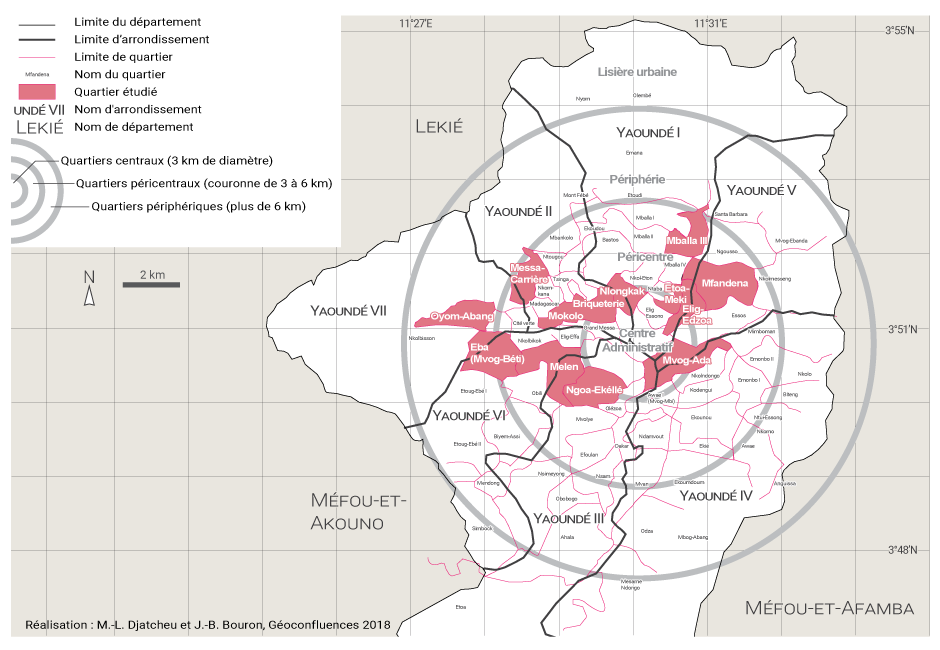
\includegraphics[width=0.8\linewidth]{Images/localisation-yaounde.png}
    \caption{architechture reseau ville de yaounde}
\end{figure}

\newpage
-Parlons maintenant des differents algorithmes de parcours qui nous interessent:
\subsubsection*{Parcours en Largeur (BFS - Breadth First Search)}
\begin{itemize}
    \item \textbf{Principe} : Le BFS explore les nœuds du graphe en utilisant un ordre de visite en largeur. Il commence par le nœud de départ, puis visite tous ses voisins avant de passer aux voisins de ces voisins, et ainsi de suite.
    \item \textbf{Spécificités} :
        \begin{itemize}
            \item Utilise une file (FIFO) pour gérer l'ordre de visite des nœuds.
            \item Trouve le plus court chemin entre deux nœuds non pondérés.
            \item Convient pour la recherche de la solution la plus rapide.
        \end{itemize}
\end{itemize}

\begin{figure}[h]
    \centering
    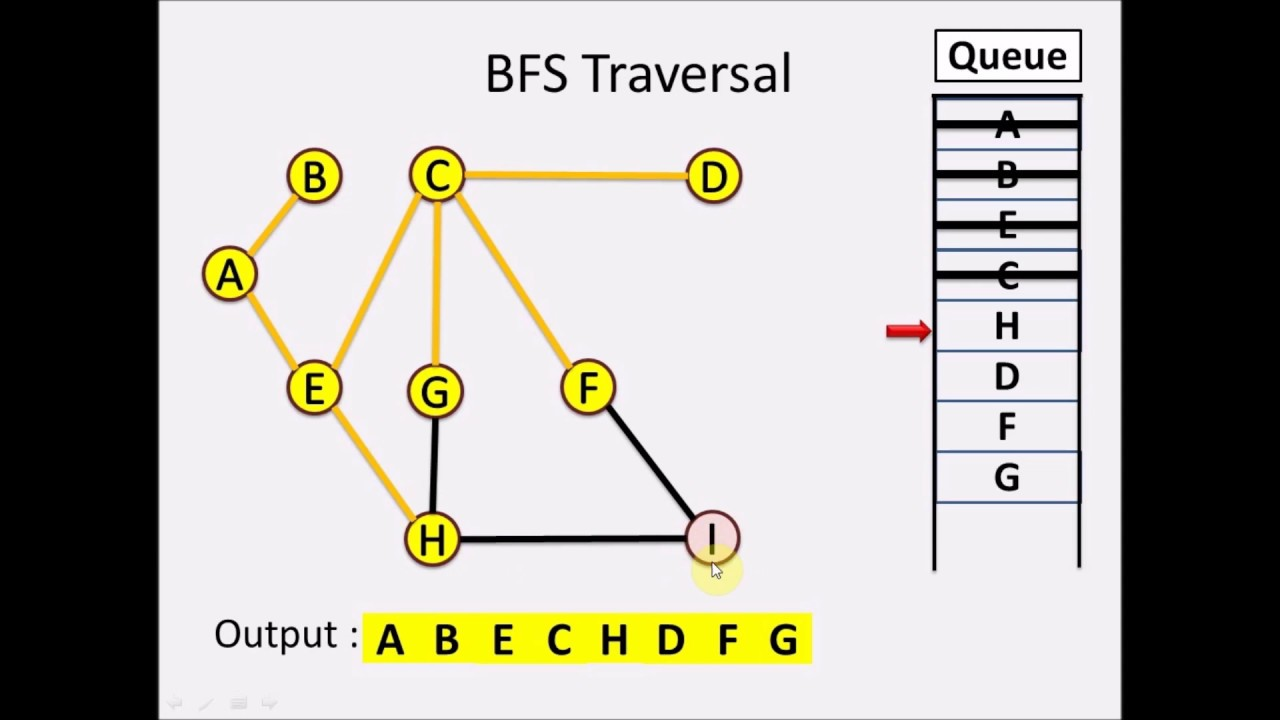
\includegraphics[width=0.5\linewidth]{Images/BFS.jpeg}
    \caption{algorithme BFS}
\end{figure}


\subsubsection*{Parcours en Profondeur (DFS - Depth First Search)}
\begin{itemize}
    \item \textbf{Principe} : Le DFS explore les nœuds du graphe en utilisant la récursivité. Il visite les nœuds les plus "profonds" en premier, puis remonte progressivement dans le graphe.
    \item \textbf{Spécificités} :
        \begin{itemize}
            \item Utilise la pile (LIFO) pour gérer l'ordre de visite des nœuds.
            \item Peut être utilisé pour détecter des cycles dans un graphe.
            \item Ne garantit pas le plus court chemin.
        \end{itemize}
\end{itemize}

\begin{figure}[h]
    \centering
    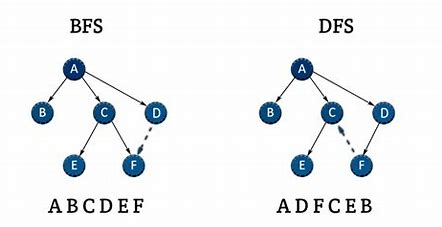
\includegraphics[width=0.5\linewidth]{Images/DFS.jpeg}
    \caption{algorithme DFS}
\end{figure}

\subsubsection*{Algorithme de Dijkstra}
\begin{itemize}
    \item \textbf{Principe} : L'algorithme de Dijkstra permet de trouver le plus court chemin entre deux sommets d'un graphe (orienté ou non orienté). Il choisit le sommet non visité avec la distance la plus faible, calcule la distance à travers lui pour chaque voisin non visité, et met à jour la distance du voisin si elle est plus petite.
    \item \textbf{Spécificités} :
        \begin{itemize}
            \item Utilise un tableau de mémoire pour garder en mémoire les distances minimisées.
            \item Convient pour les graphes orientés pondérés par des réels positifs.
            \item Peut également calculer un plus court chemin entre un sommet de départ et un sommet d'arrivée.
        \end{itemize}
\end{itemize}

\begin{figure}[h]
    \centering
    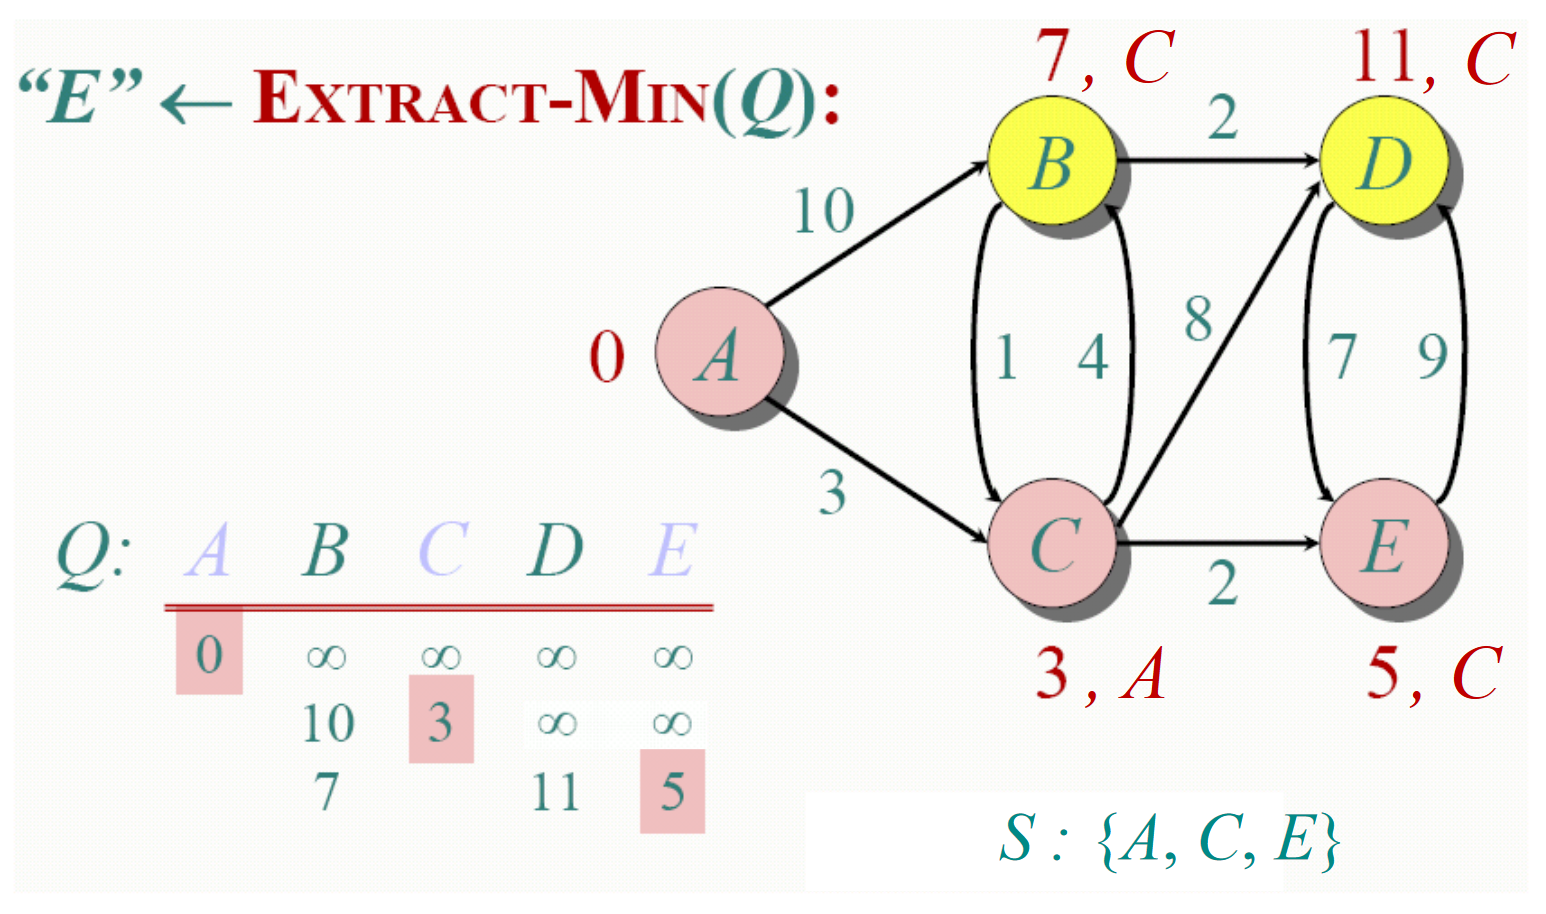
\includegraphics[width=0.5\linewidth]{Images/djiskra.png}
    \caption{Algorithme de Dijkstra}
\end{figure}

\subsubsection*{Algorithme A*}

\begin{figure}[h]
    \centering
    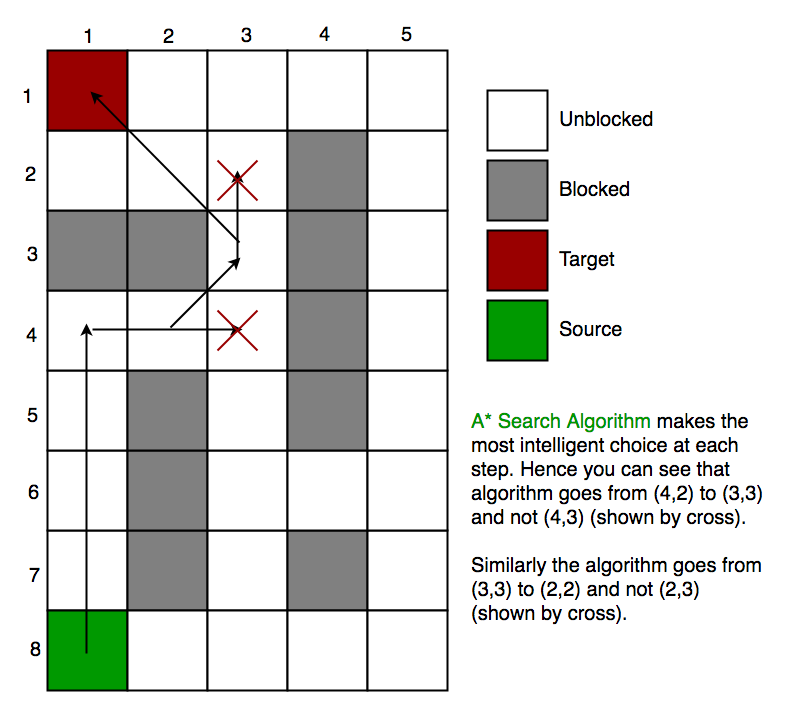
\includegraphics[width=0.5\linewidth]{Images/a_-search-algorithm-2.png}
    \caption{Algorithme A*}
\end{figure}

\begin{itemize}
    \item \textbf{Principe} : L'algorithme A* utilise une fonction heuristique pour estimer le coût restant à parcourir pour atteindre le sommet cible à partir du sommet actuel. Il combine cette estimation avec le coût réel parcouru jusqu'à présent pour évaluer les sommets à explorer en priorité. A* explore les sommets avec le coût total le plus faible en priorité.
    \item \textbf{Spécificités} :
        \begin{itemize}
            \item Utilisation d'une fonction heuristique : L'algorithme A* utilise une fonction heuristique qui fournit une estimation du coût restant pour atteindre le sommet cible. Cette fonction doit être admissible (ne jamais surestimer le coût restant) pour garantir l'optimalité de l'algorithme.
            \item Efficace pour la recherche de chemins dans les graphes avec des coûts non uniformes : L'algorithme A* peut être plus efficace que Dijkstra dans les graphes où les coûts des arêtes varient et nécessitent une exploration plus intelligente.
        \end{itemize}
\end{itemize}


En résumé, le choix de l'algorithme dépend du problème spécifique que vous essayez de résoudre. Le BFS est idéal pour les chemins les plus courts, tandis que le DFS est plus souple pour explorer toutes les possibilités. L'algorithme de Dijkstra est puissant et polyvalent pour résoudre les problèmes de plus court chemin. L'algorithme A*, quant à lui, offre une approche efficace pour trouver des chemins dans les graphes avec des coûts non uniformes, en utilisant une fonction heuristique pour guider la recherche. Celui que nous allons souvent utiliser dépendra à chaque fois de la tâche que nous voudrons accomplir lors de la gestion des sommets sur notre graphe.





